\section{Problem 3}
\label{part3}
\begin{verbatim}
Using D3, create a graph of the Karate club before and after
the split.

- Weight the edges with the data from: 
http://vlado.fmf.uni-lj.si/pub/networks/data/ucinet/zachary.dat

- Have the transition from before/after the split occur on a mouse
click.  This is a toggle, so the graph will go back and forth beween
connected and disconnected.
\end{verbatim}
\subsection{Solution}
\begin{enumerate}

\item This question is similar to the previous assignment. In previous assignment I created the graph using python library and now with d3.js.
\item The first step here is to convert the GraphML file into json file so that i can give the json file as input to my Html code.
\item The sample graphMl file can be seen in figure\ref{Sample3_t1}.
\item I wrote a python code for converting the graphMl to json and that code can be seen here in listing\ref{lst:q3-1}.
\item I used ``BeautifulSoup'' in order to get the data from the GraphML and the final sample json file can be viewed here in figure\ref{Sample3_t2}.
\item This json file is given as input to the Html code which can be seen here in listing\ref{lst:q3-2}.
\item In order to toggle between before and after split graphs, I inserted buttons and the sample graphs can be seen here in figure\ref{graph3} and figure\ref{graph4}.
\item The working model of d3 graph can be viewed in this link \url{http://bl.ocks.org/PaladhiDinesh/617c3ef60a692d2f972a}.

\newpage
\end{enumerate}
\subsection{Code Listing}

\lstinputlisting[language=Python,breaklines = true,frame=single,caption={Python Code for converting graphml to json}, label=lst:q3-1,captionpos=b,numbers=left,showspaces=false,showstringspaces=false,basicstyle=\footnotesize]{graphml_tojson.py}
\newpage

\subsection{Code Listing}

\lstinputlisting[language=Html,breaklines = true,frame=single,caption={HTML code with d3 to get force directed graph}, label=lst:q3-2,captionpos=b,numbers=left,showspaces=false,showstringspaces=false,basicstyle=\footnotesize]{node_link.html}
\newpage

\subsection{Results}

\begin{figure}[ht]    
    \begin{center}
        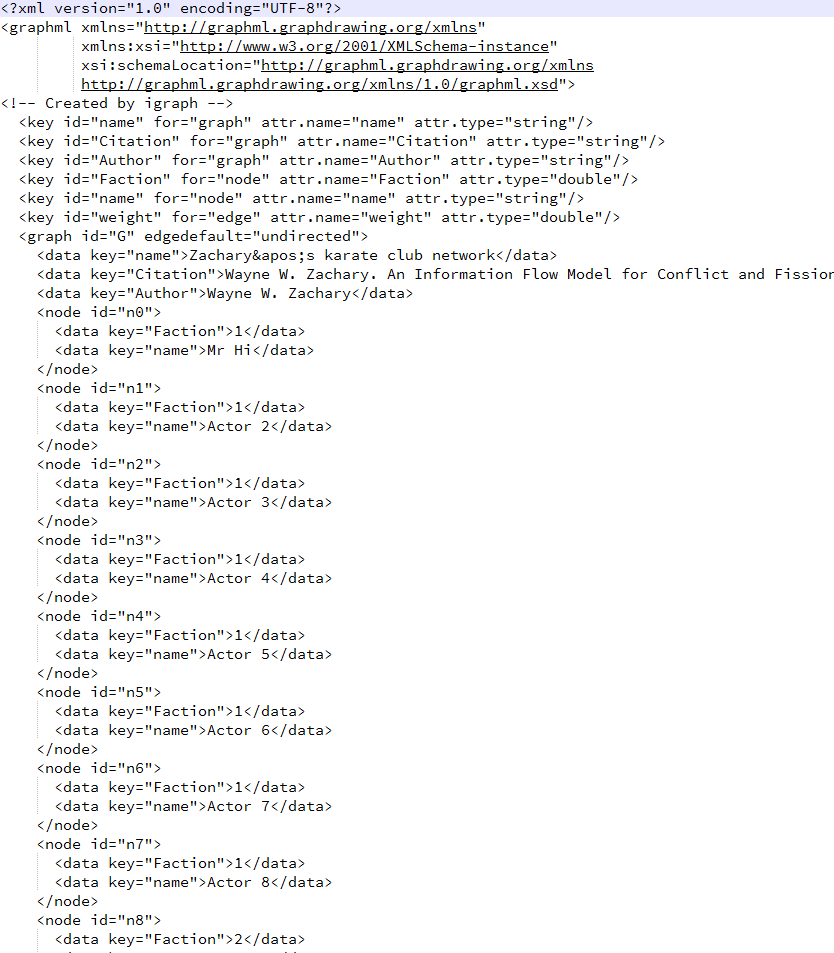
\includegraphics[scale=0.7]{q3_sample_graphml.png}
        \caption{Sample GraphML file for karate club}
        \label{Sample3_t1}
    \end{center}
\end{figure}
\newpage
\subsubsection{Final json}
\begin{figure}[ht]    
    \begin{center}
        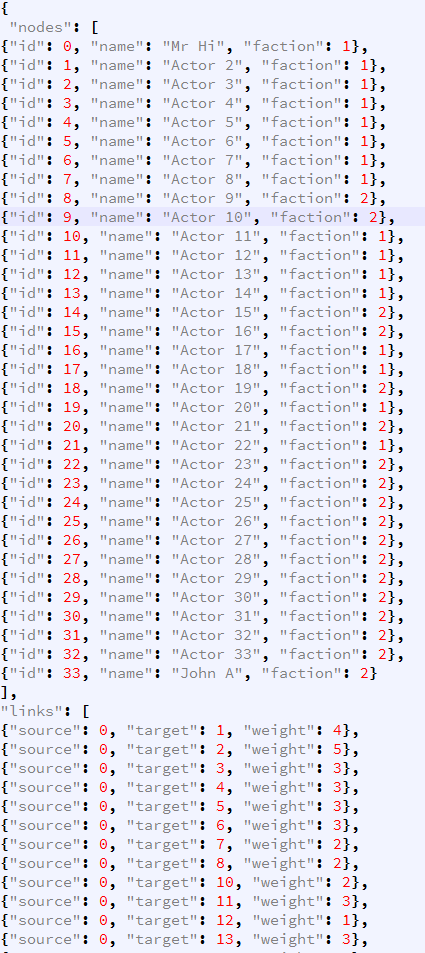
\includegraphics[scale=0.6]{q3_sample_json.png}
        \caption{Sample Final json }
        \label{Sample3_t2}
    \end{center}
\end{figure}
\newpage

\subsubsection{D3 Graph}
\begin{figure}[ht]    
    \begin{center}
        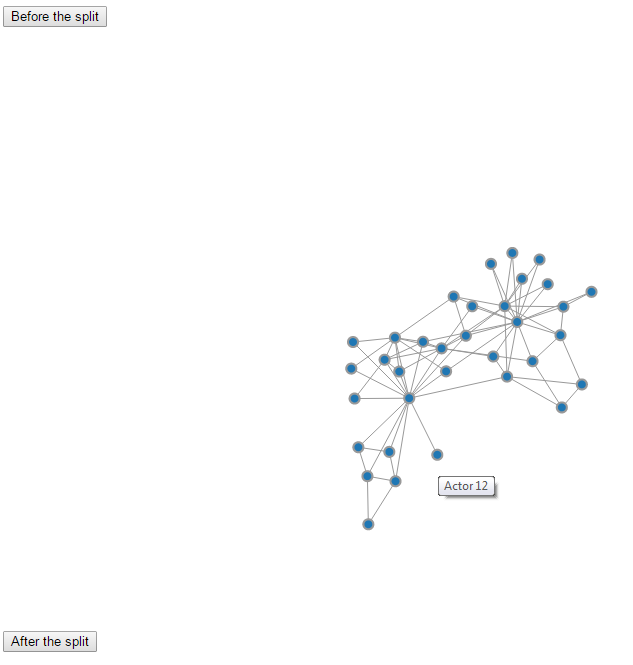
\includegraphics[scale=0.4]{q3_before.png}
        \caption{D3 Graph before split}
        \label{graph3}
    \end{center}
\end{figure}
\subsubsection{D3 Graph}
\begin{figure}[ht]    
    \begin{center}
        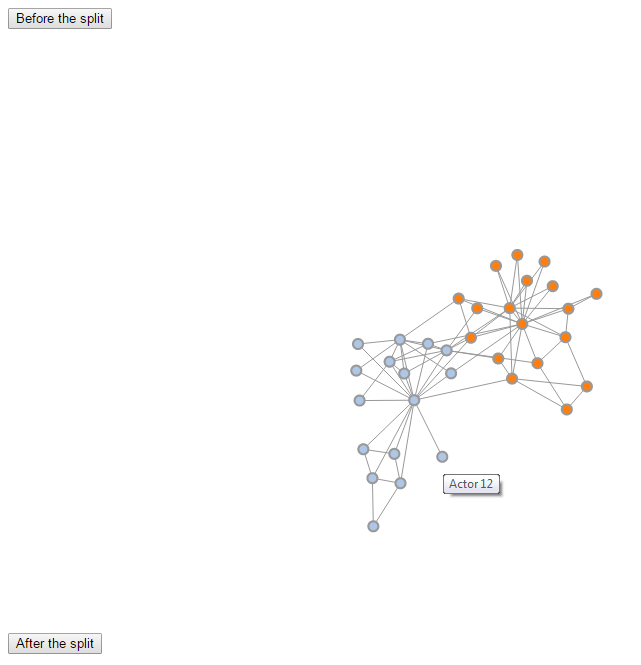
\includegraphics[scale=0.4]{q3_after.png}
        \caption{D3 Graph after split}
        \label{graph4}
    \end{center}
\end{figure}
\newpage

